\begin{figure}[t!]
  \centering
  \begin{minipage}{0.49\textwidth}
    \centering
    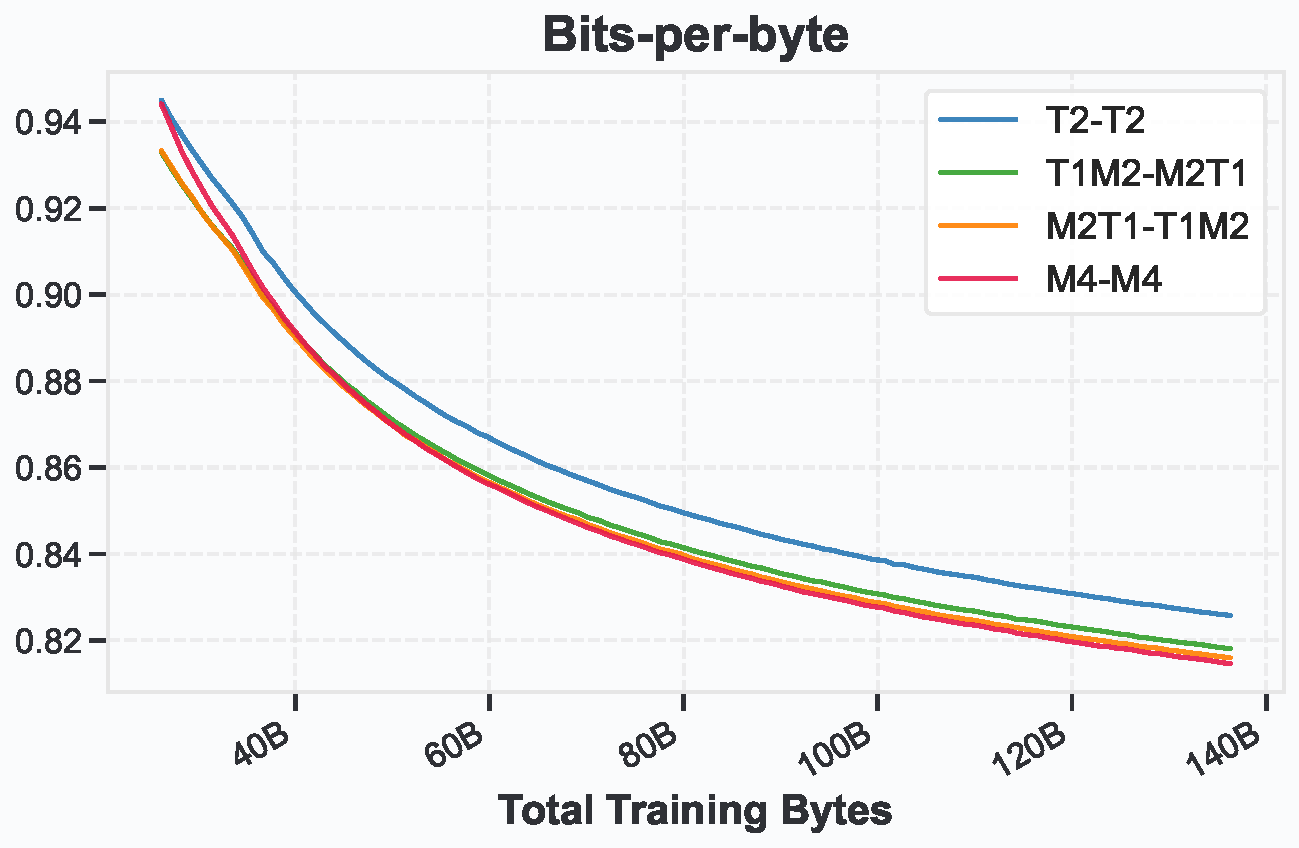
\includegraphics[width=\linewidth]{fig_img/abl_enc_dec_combination_spacebyte.pdf}
    \captionof{figure}{
        \textbf{SpaceByte++ encoder-decoder architecture ablation using raw byte inputs.}
        We evaluate four encoder-decoder ($\mathcal{E}^0-\mathcal{D}^0$) configurations: M4-M4 , M2T1-T1M2 and T1M2-M2T1, and T2-T2, where M denotes Mamba layers and T denotes Transformer layers.
    }
    \label{fig: abl_enc_dec_combination_spacebyte}
  \end{minipage}
  \hfill
  \begin{minipage}{0.49\textwidth}
    \centering
    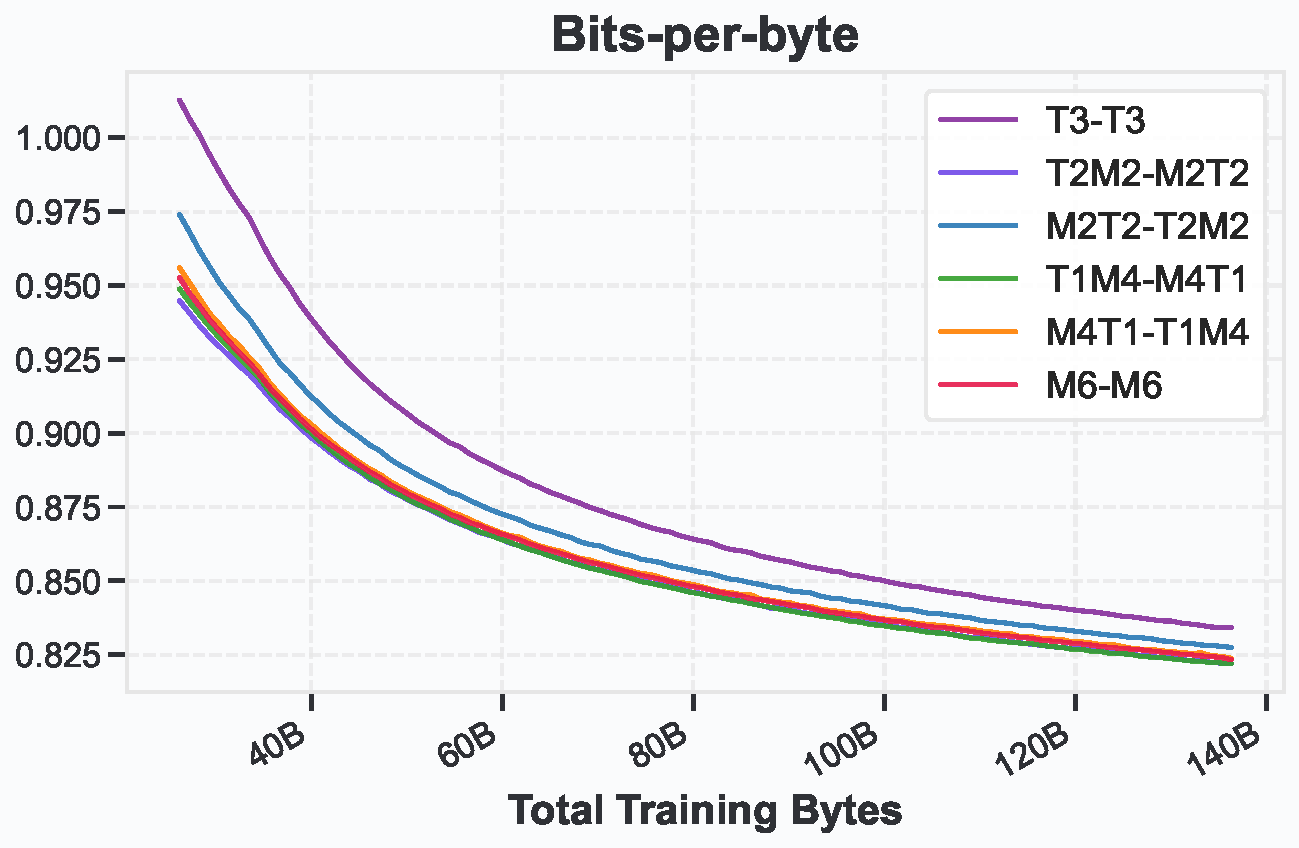
\includegraphics[width=\linewidth]{fig_img/abl_enc_dec_combination_BPE.pdf}
    \captionof{figure}{
        \textbf{Encoder-decoder architecture ablation using BPE-tokenized inputs.}
        Assuming that GPT-2 tokenizer serves as the outermost encoder-decoder (\ie{} $\mathcal{E}^0$-$\mathcal{D}^0$), we evaluate six $\mathcal{E}^1$-$\mathcal{D}^1$ combinations: M6-M6, M4T1-T1M4, T1M4-M4T1, M2T2-T2M2, T2M2-M2T2, and T3-T3.
    }
    \label{fig: abl_enc_dec_combination_BPE}
  \end{minipage}
\end{figure}
